% vim: set filetype=tex

\section{\color{fancy}Chapter 7: Histogram}

\begin{figure}[h]
  \centering
  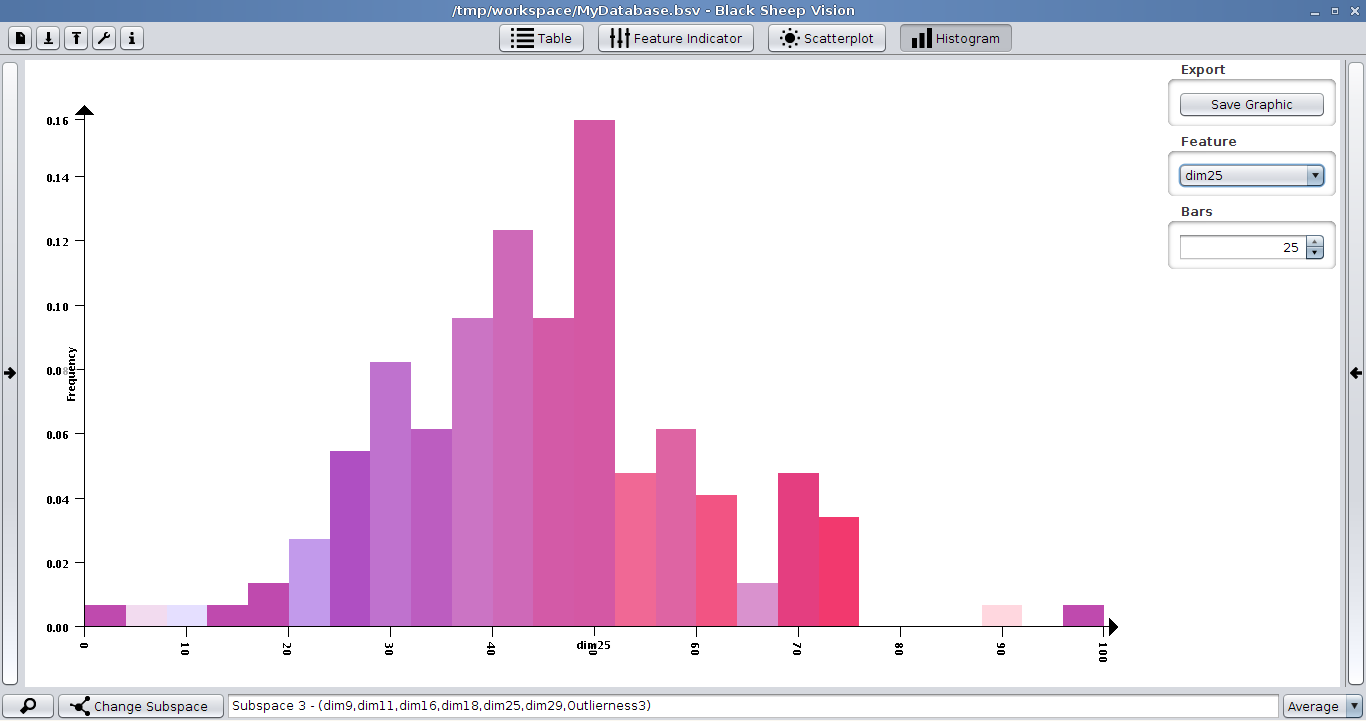
\includegraphics[width=16cm]{images/bsv/Histogram.png}
  \caption{Histogram}
  \label{fig:histogram}
\end{figure}

\subsection{Functionality}
\begin{tabular}{p{0.2\linewidth}p{0.7\linewidth}}
  \color{fancy}Feature & \color{fancy}Usage \\ \hline
  Display & The Histogram shows the distribution of your data for one feature at a time. \\ \hline
  Control & On the right side you find the control menu, which lets you export the current view (e.g. as a \textbf{.svg}), specify the feature to plot or set the number of bars to plot, in order to better control the visualization of peaks in your data. \\ \hline
  Select & You are able to select the feature, for which the distribution is to be shown, by selecting it in the control menu. \\ \hline
\end{tabular}

\subsection{Shortcuts}
There are no shortcuts defined for this view, in the current version.
